    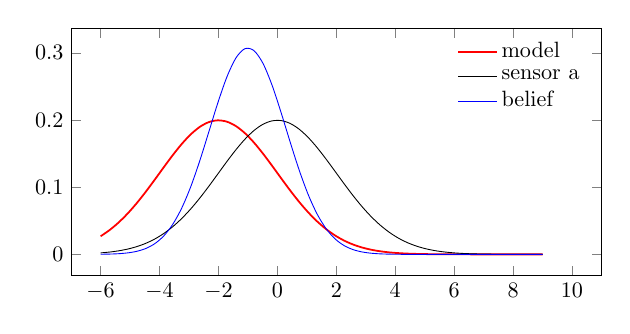
\begin{tikzpicture}[
      declare function={
        normalpdf(\x,\mu,\sigma)=
        (2*3.1415*\sigma^2)^(-0.5)*exp(-(\x-\mu)^2/(2*\sigma^2));
      },
      hplot/.style={ycomb, mark=o, dashed}, ,scale=0.8]
    
      \begin{axis}[
        width=10cm, height=5.5cm,
        samples=50,
        legend style={draw=none, fill=none},
        domain=-6:9,
        legend cell align=left,
        xmin=-7, xmax=11]
    
        \addplot [smooth, thick, red] {normalpdf(x,-2,2)} node[] {};
        \addplot [smooth, black]      {normalpdf(x,0,2)} node[] {};
        \addplot [smooth, blue]       {normalpdf(x,-1,1.3)} node[] {};
        \legend{model, sensor a, belief};
      \end{axis}
    \end{tikzpicture}